\begin{frame}[fragile]{Proposed Method}
\vspace{-0.6cm}

\begin{center}
\begin{tikzpicture}[scale=0.75, every node/.style={scale=0.75}, node distance = 2cm, auto]

  \node [outer sep=0cm] (environment) at (0,0)  {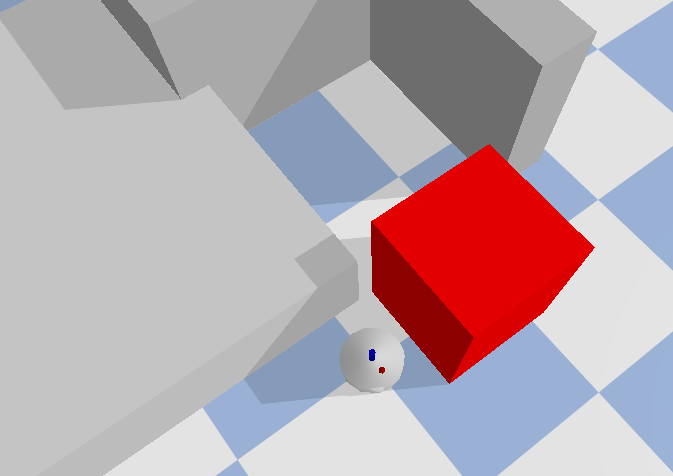
\includegraphics[width=4.6cm]{figures/introduction/robot_no_target}};

  \draw [myEvenLighterColor,
  rounded corners=0.3cm,
  line width=0.3cm]
  (environment.north west) --
  (environment.north east) --
  (environment.south east) --
  (environment.south west) -- cycle  ;

  \node [block,
  above of=environment,
  minimum height=2cm,
  minimum width=5cm,
  node distance=4.1cm,
  outer sep=0cm] (hgraph) {Hypothesis Algorithm};

  \node [block,
  above of=hgraph,
  node distance=3.3cm,
  minimum width=5cm,
  minimum height=2.0cm] (kgraph) {Knowledge Graph};

  % Draw edges
  \draw[-stealth] ([yshift=0.155cm, xshift=0.4 cm]environment.north) -- node [xshift=-.05cm, right] {\shortstack[]{sensor\\measurements}}([xshift=0.4 cm]hgraph.south) ;
  \draw[-stealth] ([xshift=-0.4 cm]hgraph.south) -- node [left] {robot input}([yshift=0.155cm, xshift=-0.4 cm]environment.north) ;
  \draw[stealth-] (hgraph.west) -- node [above] {task} ++(-1, 0);


  \draw[-stealth] ([xshift=-0.4cm]kgraph.south) -- node [left] {\shortstack[]{action\\suggestions}}([xshift= -0.4cm]hgraph.north) ;
  \draw[stealth-] ([xshift=0.4cm]kgraph.south) -- node [right] {\shortstack[]{action\\feedback}}([xshift= 0.4cm]hgraph.north) ;
\end{tikzpicture}
\end{center}

\end{frame}


\begin{frame}[fragile]{Proposed Method: K-Graph}
  \begin{figure}
    \centering
  \subfloat{ 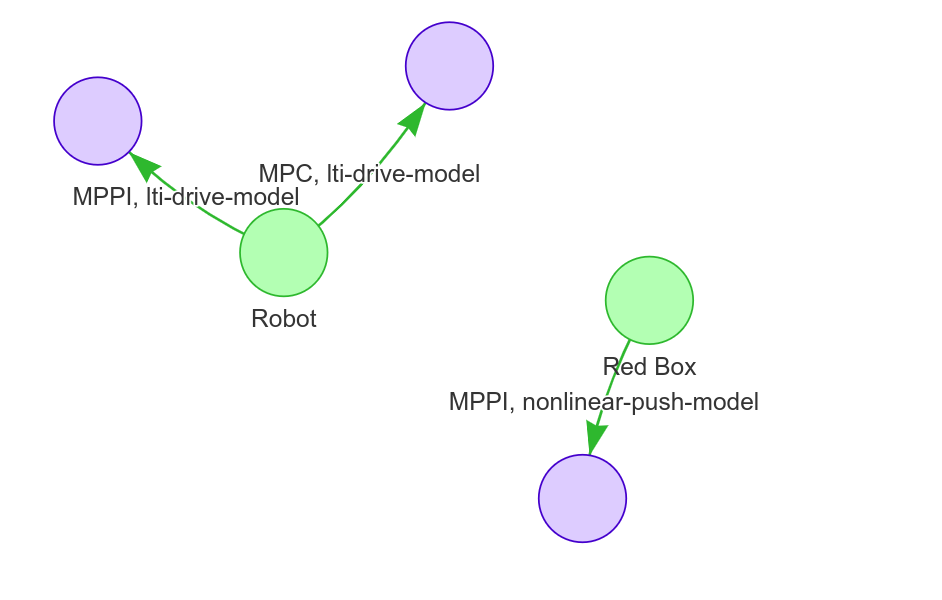
\includegraphics[height=0.8\textheight]{figures/proposed_method/kgraph_testing_phase} }
  \subfloat{ 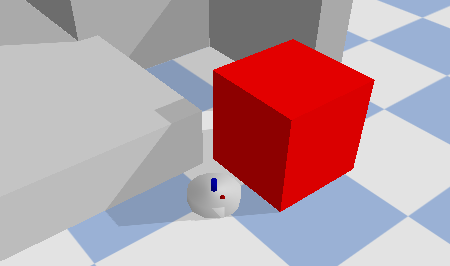
\includegraphics[height=0.3\textheight]{figures/introduction/example_env}}
\end{figure}
\end{frame}

\begin{frame}[fragile]{Proposed Method: K-Graph}
  \begin{figure}
    \centering
  \subfloat{ 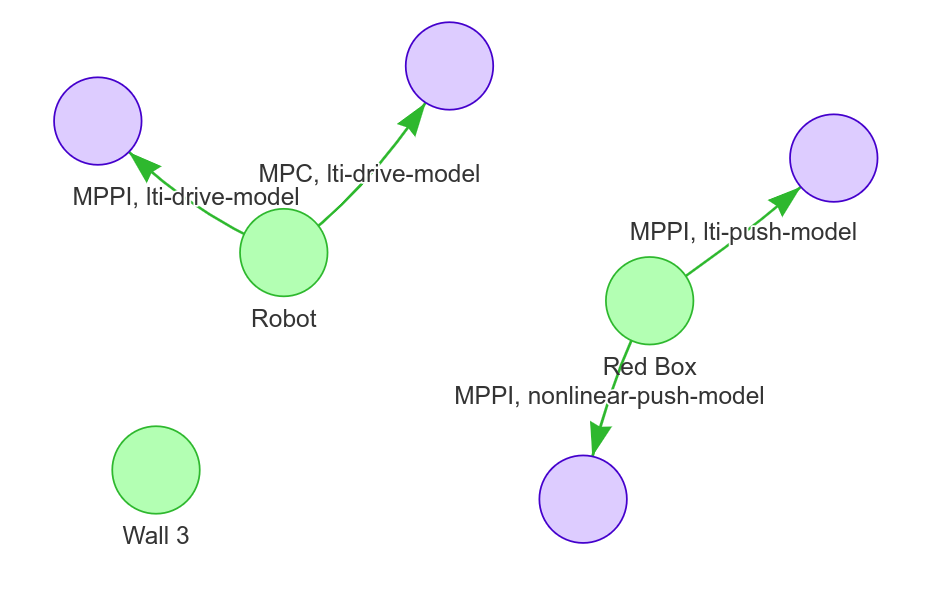
\includegraphics[height=0.8\textheight]{figures/proposed_method/kgraph_converging_phase} }
  \subfloat{ 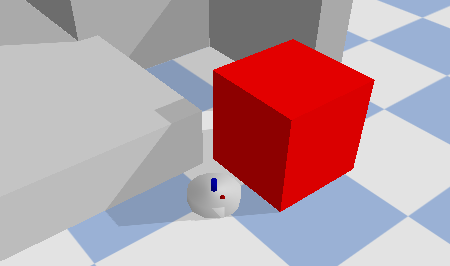
\includegraphics[height=0.3\textheight]{figures/introduction/example_env}}
\end{figure}
\end{frame}

% \begin{frame}[fragile]{Proposed Method: K-Graph}
% Formally, a \textbf{\acl{k-graph}}, $\gls{k-graph} = \left\langle \gls{nodesK}, \gls{edgesK} \right\rangle $
% \\comprising $\gls{nodesK} = \{\gls{node}^{\mathit{center}}, \gls{node}^{\mathit{side}}\}$, \quad $\gls{edgesK} \in \{\gls{edge}_{(i,j)}| i \in \gls{nodesK}^\mathit{center}_\mathit{ids}, j \in \gls{nodesK}^\mathit{side}_\mathit{ids} \}$.\bs
% \end{frame}


\begin{frame}[fragile]{Proposed Method: K-Graph}
  % 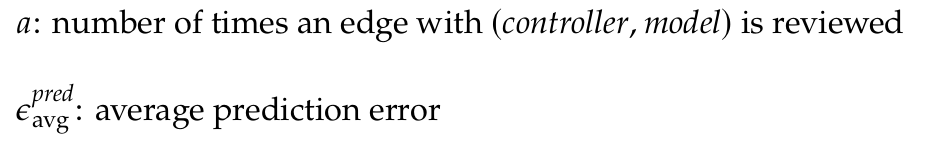
\includegraphics[width=0.8\textwidth]{figures/proposed_method/explain_successf}\pause
 $a$: number of times (\textit{controller}, \textit{model}) received action feedback\bs

 ${\epsilon^\mathit{pred}}_{avg}$: average prediction error\bs

  Action Feedback $\alpha$:\bs

  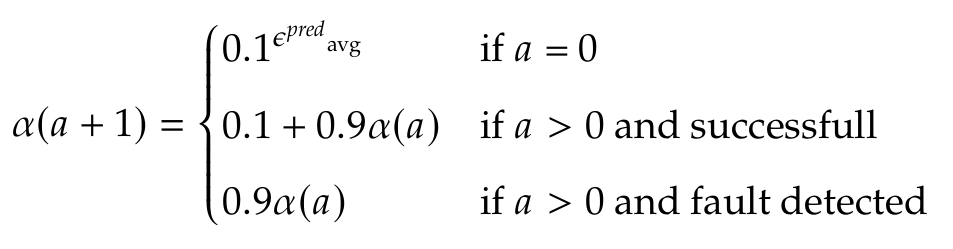
\includegraphics[width=0.7\textwidth]{figures/proposed_method/successfactor}
\end{frame}
